\section{Results}

\subsection{Comparison of the deregulated pathwways in the PDCL with the TCGA-GBM datasets}

\subsubsection{Pathways mainly involved in the Cell-Cycle, DNA replication and Repair are shared between the two datasets}

The entry \textit{Glioma} pathway (\textbf{path:hsa05214}) in \acrshort{kegg} document some of the deregulation caused by glioblastoma.
Zyla \textit{et al} used this entry as a target pathway to assess the sensitivity of different ranking metrics when studying microarray data from brain tissue \cite*{Zyla2017}.
\acrshort{fdr} value in G:Profiler is $8.898 \times 10^{-3}$ and $5.240 \times 10^{-2}$ respectively for \acrshort{pdcl} and \acrshort{tcga}, \acrshort{fdr} in \acrshort{gsea} is $4.487 \times 10^{-3}$ and $8.298 \times 10^{-1}$ respectively for \acrshort{pdcl} and \acrshort{tcga}.
Not only the \acrshort{fdr} value is lower for the \acrshort{tcga} dataset but the \acrshort{fdr} of \acrshort{gsea} for \acrshort{pdcl} does not pass the more lenient threshold we defined in this study.
Controls for the \acrshort{pdcl} dataset are taken from another study \cite*{Lundin2018}, this introduce variability not caused by deregulation of genes but more likely variability between samples or experimental conditions, while in the \acrshort{tcga} dataset controls comes from matching samples and follows the exact same protocol.
This might explain why the Glioma pathway is higher in the \acrshort{pdcl} dataset.

45 pathways are found deregulated in the \acrshort{pdcl} dataset and 304 in the \acrshort{tcga} dataset.
As can be seen in the figure \ref{fig:heatmap-fdr-global-tcga}, the two datasets shared 19 significantly deregulated pathways which are involved in the cell-cycle, DNA repair and replication, gene expression, extracellular matrix and in diseases.
\begin{figure}
    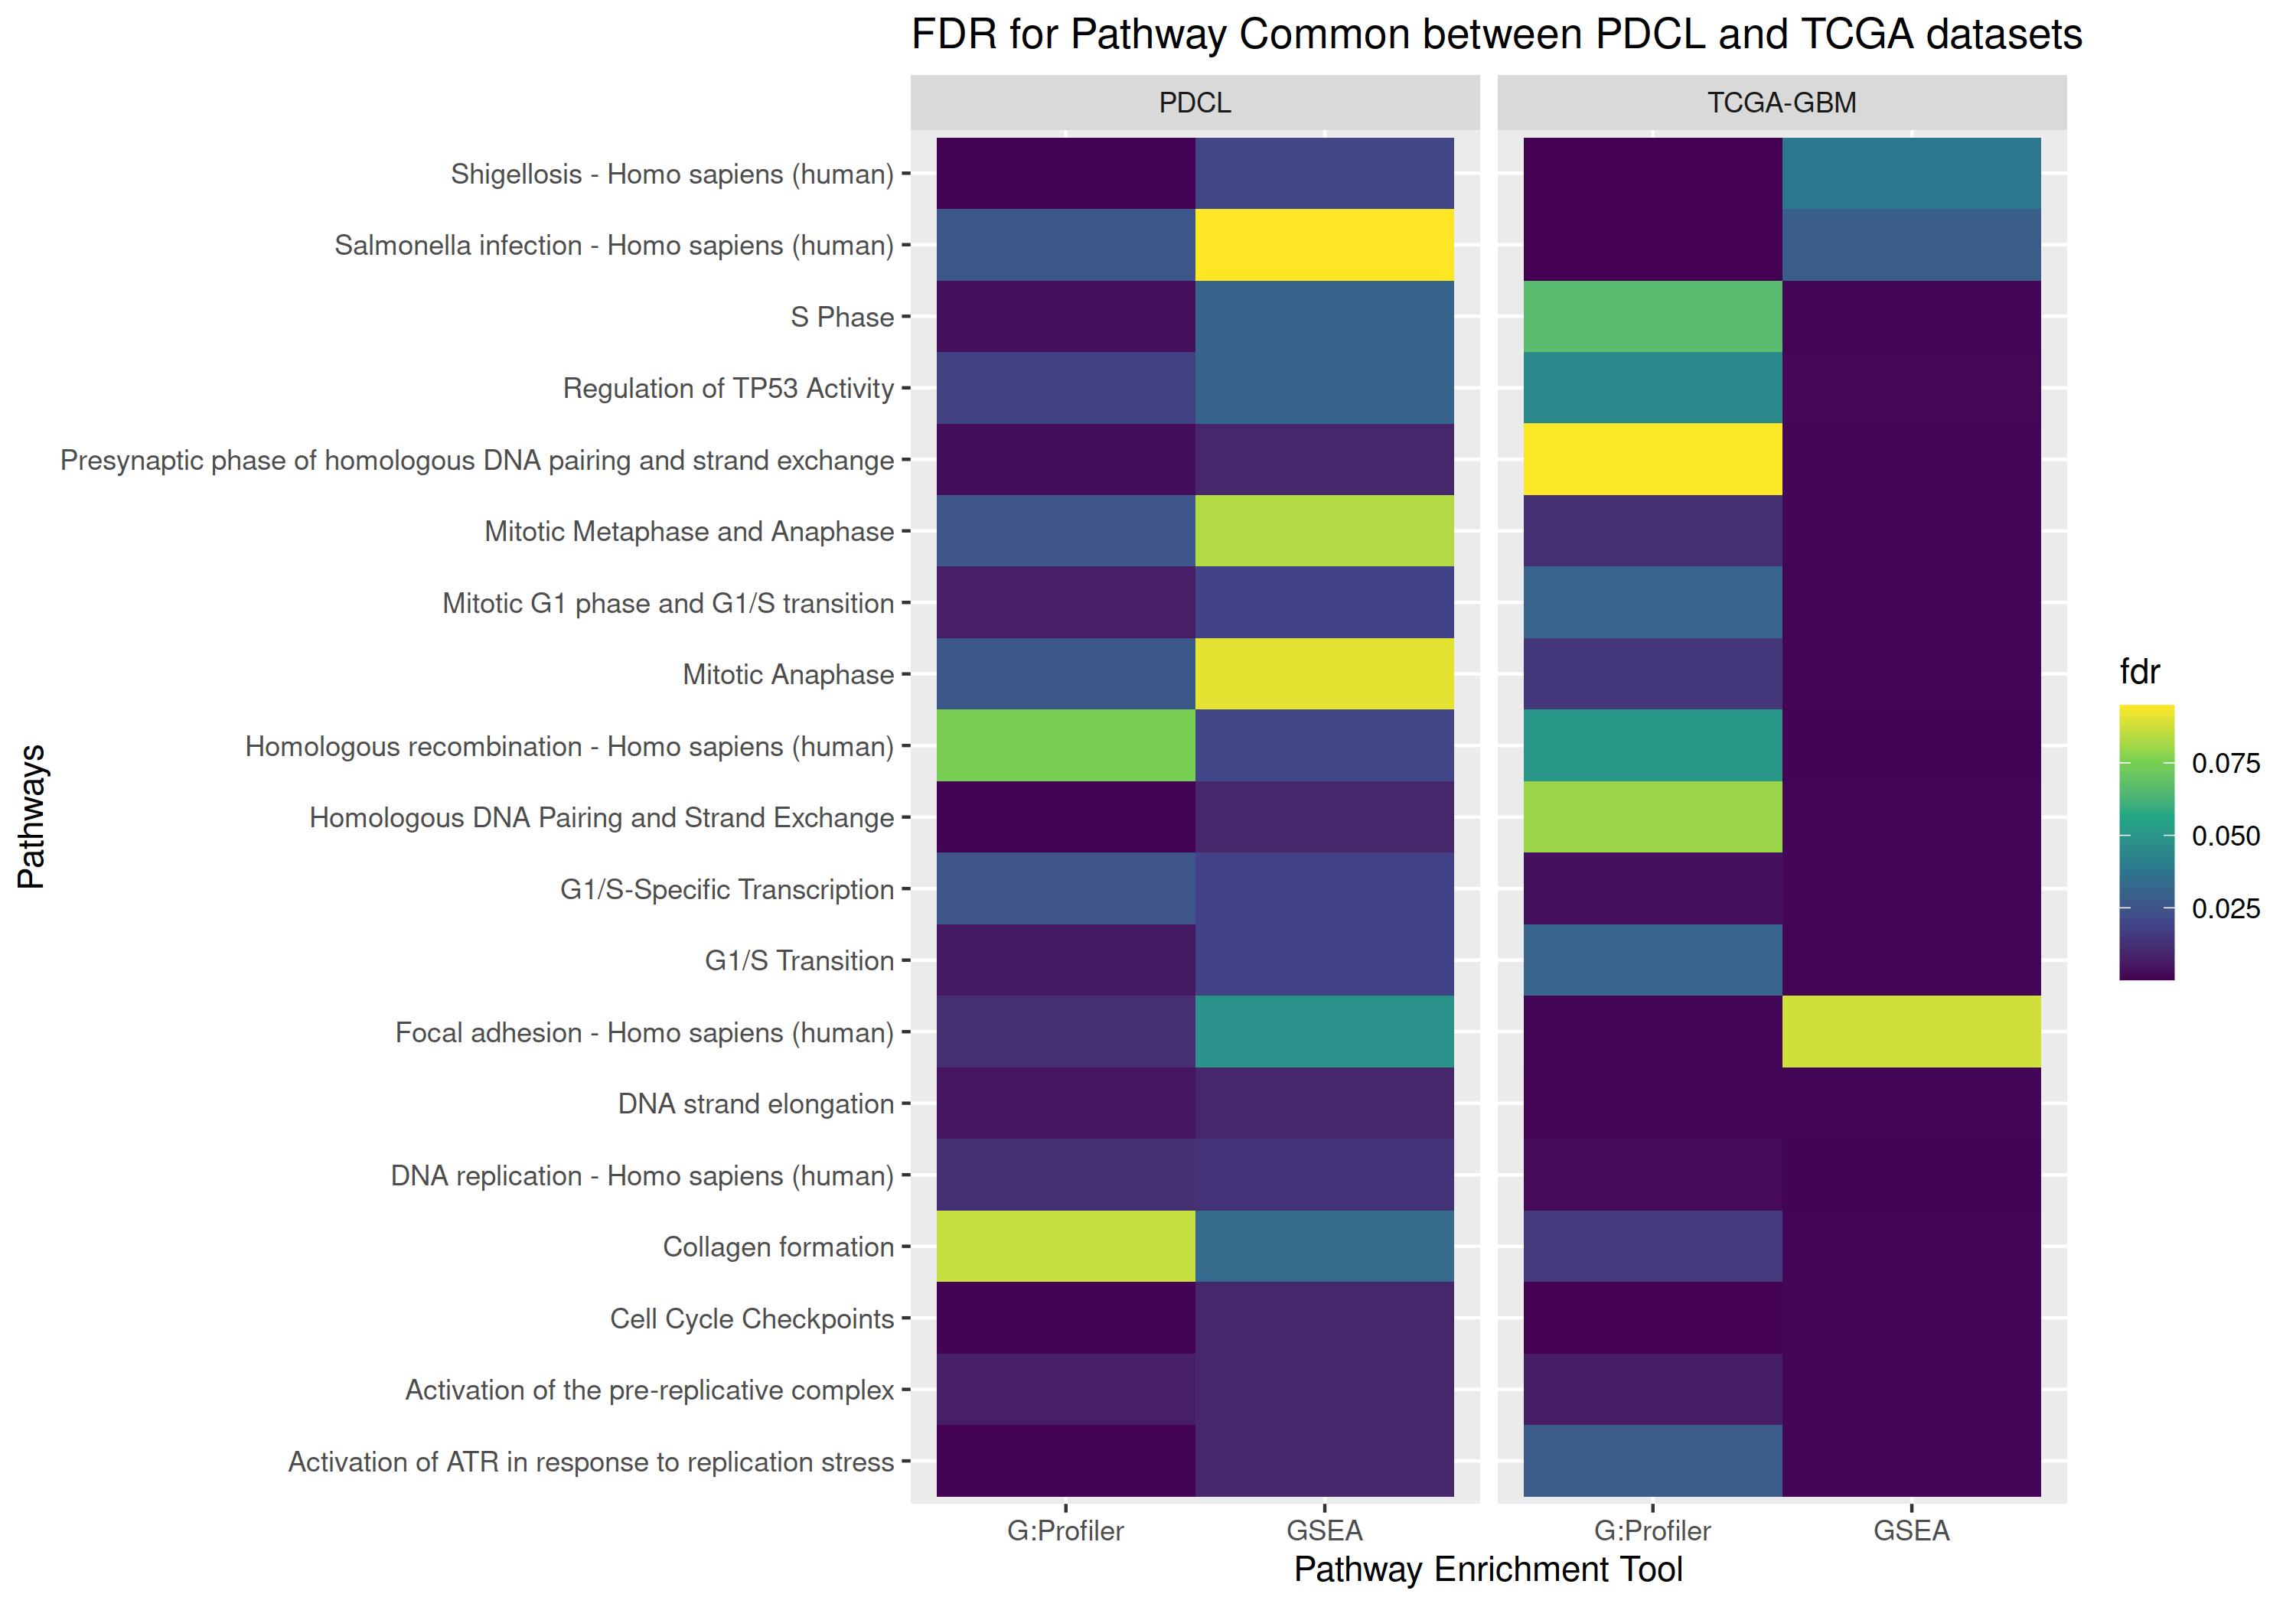
\includegraphics[width=\textwidth]{img/heatmap-fdr-global-tcga}
    \caption{
        \acrfull{fdr} of the pathways deregulated in both the \acrshort{pdcl} and the \acrshort{tcga} datasets.
        \acrshort{fdr} is lower than 0.1 since we only keep pathways that below this value.
    }
    \label{fig:heatmap-fdr-global-tcga}
\end{figure}
The 2 pathways associated with disease (Shigellosis and Salmonella infection) belong to the \acrshort{kegg} database.
However, pathways involved in DNA replication and repair are significantly enriched for both \acrshort{kegg} and Reactome.
Interestingly, the shared pathway \textit{Regulation of TP53 activity} is found upregulated by \acrshort{gsea} for both datasets.
A study from \acrshort{tcga} on frequent mutations in glioblastoma has showed that p53 signaling is altered  in 87\% of the samples and p53 is inactivated by mutation in 35\% of the samples \cite*{McLendon2008}.
Thus, regulation of p53 may be upregulated to make up for the lack of activity from the mutated p53.

Among the pathways enriched only in thez \acrshort{tcga} dataset, we found pathways that are children of the shared pathways between both dataset.
For example, \textit{Amplification of signal from unattached kinetochores via a MAD2 inhibitory signal} (R-HSA-141444) is a children pathway of \textit{Cell Cycle Checkpoints} (R-HSA-69620) that is to say it is smaller pathway which take place in its parent pathways.
When we compared the \acrshort{fdr} values of this pathways in G:Profiler and \acrshort{gsea} for both dataset, only G:Profiler's result does not pass the threshold used (\acrshort{fdr} value is 0.125 in G:Profiler with \acrshort{pdcl} sample).
Although almost all genes of this pathway are present in the dataset, a closer look at the number of deregulated genes involved in this pathway in G:Profiler's result for both datasets showed 74 genes in the \acrshort{tcga} compared to 48 for \acrshort{pdcl}.
If we first hypothetized that the lower number of genes included in the \acrshort{pdcl} dataset (~20,000 genes compared to ~60,000 in \acrshort{tcga}) may reduce the ability of pathway enrichment tools to detect smaller pathways, this shows that it is rather caused by the absence of deregulation in \acrshort{pdcl} samples.

\subsubsection{Cell-Cycle}

Two phases of the Cell Cyle are enriched in both datasets : the \textit{S phase} (\textbf{R-HSA-69242}) and the \textit{Mitotic Anaphase} (\textbf{R-HSA-68882}).
Interestingly, the \textit{Mitotic Anaphase}  was enriched only in \acrshort{tcga} when we kept pathways between 15 and 1,000 genes but was enriched as well in the \acrshort{pdcl} dataset when we set up a limit of 15 to 500 genes.
This indicates that the number of pathways present in the \acrshort{gmt} file has an impact on the \acrshort{fdr} associated with each pathways.
Linked to the \textit{S phase}, the \textit{G1/S phase transition} (\textbf{R-HSA-69205}) and the \textit{DNA strand elongation} (\textbf{R-HSA-69190}) are enriched with the \textit{DNA strand elongation} a child pathway of the \textit{S phase}.
The \textit{Cell Cycle Checkpoints} pathway (\textbf{R-HSA-69620}) is enriched in both datasets.
However, \textit{Amplification of signal from unattached kinetochores via MAD2 inhibitory singal} (\textbf{R-HSA-141444}) a pathway included in the \textit{Mitotic Spindle Checkpoint} (\textbf{R-HSA-69618}) is only enriched in the \acrshort{tcga} dataset.

\subsubsection{Metabolism}

Although pathways involved in metabolism are enriched in both datasets, none of them are shared between the two dataset.
The \acrshort{tcga} dataset is mostly enriched with pathways involved in the energetic metabolism such as \textit{Phospholipid metabolism} (\textbf{R-HSA-1483257}), \textit{Regulation of insuline secretion} (\textbf{R-HSA-422356}) and \textit{Selenoamino acid metabolism} (\textbf{R-HSA-2408522}).
The glycerophospholipid metabolism, part of a phospholipid metabolism, is enriched in both Reactome and \acrshort{kegg} database.
The \acrshort{tcga} dataset is also enriched with pathways involved in the Metabolism of proteins or the Metabolism of RNA such as \textit{Peptide chain elongation} (\textbf{R-HSA-156902}), \textit{Translation initiation complex formation} (\textbf{R-HSA-72649}) and \textit{rRNA processing in the nucleus and cytosol} (\textbf{R-HSA-8868773}).
Compared to the \acrshort{tcga} dataset, there are no pathways involved in the Metabolism of proteins or the Metabolism of RNA enriched in the \acrshort{pdcl}.
Furthermore, the only pathway involved in metabolism found deregulated is the \textit{Cholesterol Biosynthesis} (\textbf{R-HSA-191273}).
In the \acrshort{kegg} database, the \textit{Steroid biosynthesis} (\textbf{path:hsa00100}) pathway, a pathway that include a set of reaction involved in the \textit{Cholesterol Biosynthesis}, is also deregulated.

\subsubsection{Extra-Cellular Matrix}

The \textit{Collagen formation} (\textbf{R-HSA-1474290}) and \textit{focal adhesion} (\textbf{path:hsa04510}) pathways are shared between the \acrshort{tcga} and \acrshort{pdcl} datasets.
They are related to the \acrlong{ecm} and the cell-matrix interactions as collagen is a protein composing the \acrshort{ecm} and the \textit{focal adhesion} is a process where the cell adhere to the matrix.
Only in the \acrshort{tcga} dataset, the \textit{Assembly of collagen fibrils and other multimeric structures} (\textbf{R-HSA-2022090}) and the \textit{Collagen biosynthesis and modifying enzymes} (\textbf{R-HSA-1650814}), two pathways included in the \textit{Collagen formation}, are found enriched.
The \textit{\acrshort{ecm}-receptor interaction} (\textbf{path:hsa04512}), \textit{Cell adhesion molecules} (\textbf{path:hsa04514}) and the \textit{Laminin interaction} (\textbf{R-HSA-3000157}) are pathways related to the adhesion of the cell to the \acrshort{ecm} only enriched in the \acrshort{tcga} datasets as well.
The \textit{Non-integrin membrane-ECM interactions} (\textbf{R-HSA-3000171}) is another pathway related to the \acrshort{ecm}-cell interactions yet only found enriched in the \acrshort{pdcl}.
The results seems to indicate that \acrshort{ecm} and cell adhesion carries a role for glioblastoma growth.
Since the \textit{Collagen formation} pathway is shared by the two datasets, it suggest that this process is important for glioblastoma growth.
However, \textit{Laminin interaction} and \textit{Non-integrin membrane-ECM interactions}, two pathways classified on the same level in the hierarchie of Reactome, tend to shows different mechanisms by which the tumour cell can influence its adhesion to the \acrshort{ecm}.

\subsubsection{Neuronal System}

\subsection{Comparison of the deregulated pathways between PDCLs}

\subsubsection{Cell adhesion to the ECM is the most frequently deregulated pathways}

In addition to a global comparison between glioblastoma and normal samples, we also compare each glioblastoma samples in the \acrshort{pdcl} dataset to assess the samples specific deregulations.
Table \ref*{table:frequently-dereg-pathways} shows the pathways found deregulated in at least 3 different \acrshort{pdcl} samples.
\textit{Focal adhesion} is the most commonly deregulated pathway with 13 different samples, slightly more than half of the total number of samples in the dataset.
It is also a deregulated pathway found shared between the \acrshort{tcga} and \acrshort{pdcl} dataset when conudcting the global.
Hence, this pathway might have potential in glioblastoma therapy for a wide range of tumour.
To corroborate this hypothesis, other pathways involved in collagen synthesis and  interactions \acrshort{ecm}-cell interactions are deregulated in 3 to 6 different samples (\textbf{R-HSA-1650814}, \textbf{path:hsa04512}, \textbf{R-HSA-8948216}, \textbf{R-HSA-1474290}).
In a similar way, \textit{Steroid biosynthesis} and \textit{Cholesterol biosynthesis}, two pathways identified in the \acrshort{pdcl} during the global analysis, are found deregulated in 5 and 3 different samples, respectively.
Despite it is not found enriched in the global analysis, the \textit{Oxidative phosphorylation} (\textbf{path:hsa00190}), well-known for its role in the generation of \acrshort{atp}, is found deregulated in 5 samples.
This pathway has been widely studied due to its important role in the generation of \acrshort{atp} and its potential implification in the Warburg Effect, an increase of usage of glycolysis to produce \acrshort{atp} even though oxygen is available.
It was first hypothetized that mitochondria were deffective in tumour cell, yet it was later mitochondrial function was similar to normal cells \cite*{Cairns2011}.
Since this pathway is not deregulated in the global anayslis yet it is in 5 different samples, the results suggest that deregulation of this process is cell-dependant rather than a common feature of cancer.
However, this process is unexpectedly up-regulated in all those 5 samples which contrast with the previous statement.
For this reason, this result should be taken carefully.
The second most frenquently deregulated patwhay is the \textit{Axon guidance} (\textbf{path:hsa04360}), a pathway involved in the formation of the neuronal network using guidance factors to influence the the way the growth cone will turn.
The \textit{Hippo signaling pathway} (\textbf{path:hsa04392}, \textbf{path:hsa04390}) and \textit{Retrograde endocannnabinoid signaling} (\textbf{path:hsa04723}), two signaling pathway whose role in cancer have been documented in the litterature, are found deregulated in 6 and 5 different samples, respectively.
\todo{read the article about them before citing them as references}

\begin{table}
    \centering
    \resizebox*{\textwidth}{!}{
        \begin{tabular}{ |c|c|c|c|c| }
            \hline
            Pathway ID & Description & Database & Category & Number of PDCL \\
            \hline
            path:hsa04510 & Focal adhesion & KEGG & Cellular Processes & 13 \\
            path:hsa04360 & Axon guidance & KEGG & Organismal Systems & 9 \\
            R-HSA-1650814 & Collagen biosynthesis and modifying enzymes & Reactome & ECM & 6 \\
            path:hsa00100 & Steroid biosynthesis & KEGG & Metabolism & 5 \\
            path:hsa00190 & Oxidative phosphorylation & KEGG & Metabolism & 5 \\
            path:hsa04392 & Hippo signaling pathway - multiple species & KEGG & Environmental Information Processing & 5 \\
            path:hsa04512 & ECM-receptor interaction & KEGG & Environmental Information Processing & 5 \\
            path:hsa04723 & Retrograde endocannabinoid signaling & KEGG & Organismal Systems & 5 \\
            R-HSA-8948216 & Collagen chain trimerization & Reactome & ECM & 5 \\
            path:hsa03008 & Ribosome biogenesis in eukaryotes & KEGG & Genetic Information Processing & 3 \\
            path:hsa03020 & RNA polymerase & KEGG & Genetic Information Processing & 3 \\
            path:hsa04390 & Hippo signaling pathway & KEGG & Environmental Information Processing & 3 \\
            path:hsa04612 & Antigen processing and presentation & KEGG & Organismal Systems & 3 \\
            path:hsa04714 & Thermogenesis & KEGG & Organismal Systems & 3 \\
            R-HSA-1474290 & Collagen formation & Reactome & ECM & 3 \\
            R-HSA-176187 & Activation of ATR in response to replication stress & Reactome & Cell Cycle & 3 \\
            R-HSA-191273 & Cholesterol biosynthesis & Reactome & Metabolism & 3 \\
            R-HSA-5693538 & Homology Directed Repair & Reactome & DNA Repair & 3 \\
            R-HSA-6790901 & rRNA modification in the nucleus and cytosol & Reactome & Metabolism of RNA & 3 \\
            \hline
        \end{tabular}
    }
    \caption{
        Table of the frequently deregulated pathways in the \acrshort{pdcl} dataset when assessing the alteration specfic to each samples.
        The table includes only pathways that found deregulated in at least three different samples, totalising 18 pathways.
        The \acrshort{kegg} database include two different entries for the \textit{Hippo signaling} pathway.
        Taken together, the \textit{Hippo signaling} pathway is found deregulated in 6 samples.
    }
    \label{table:frequently-dereg-pathways}
\end{table}

\subsubsection{Differencies in deregulated processes between PDCL samples}

\begin{figure}
    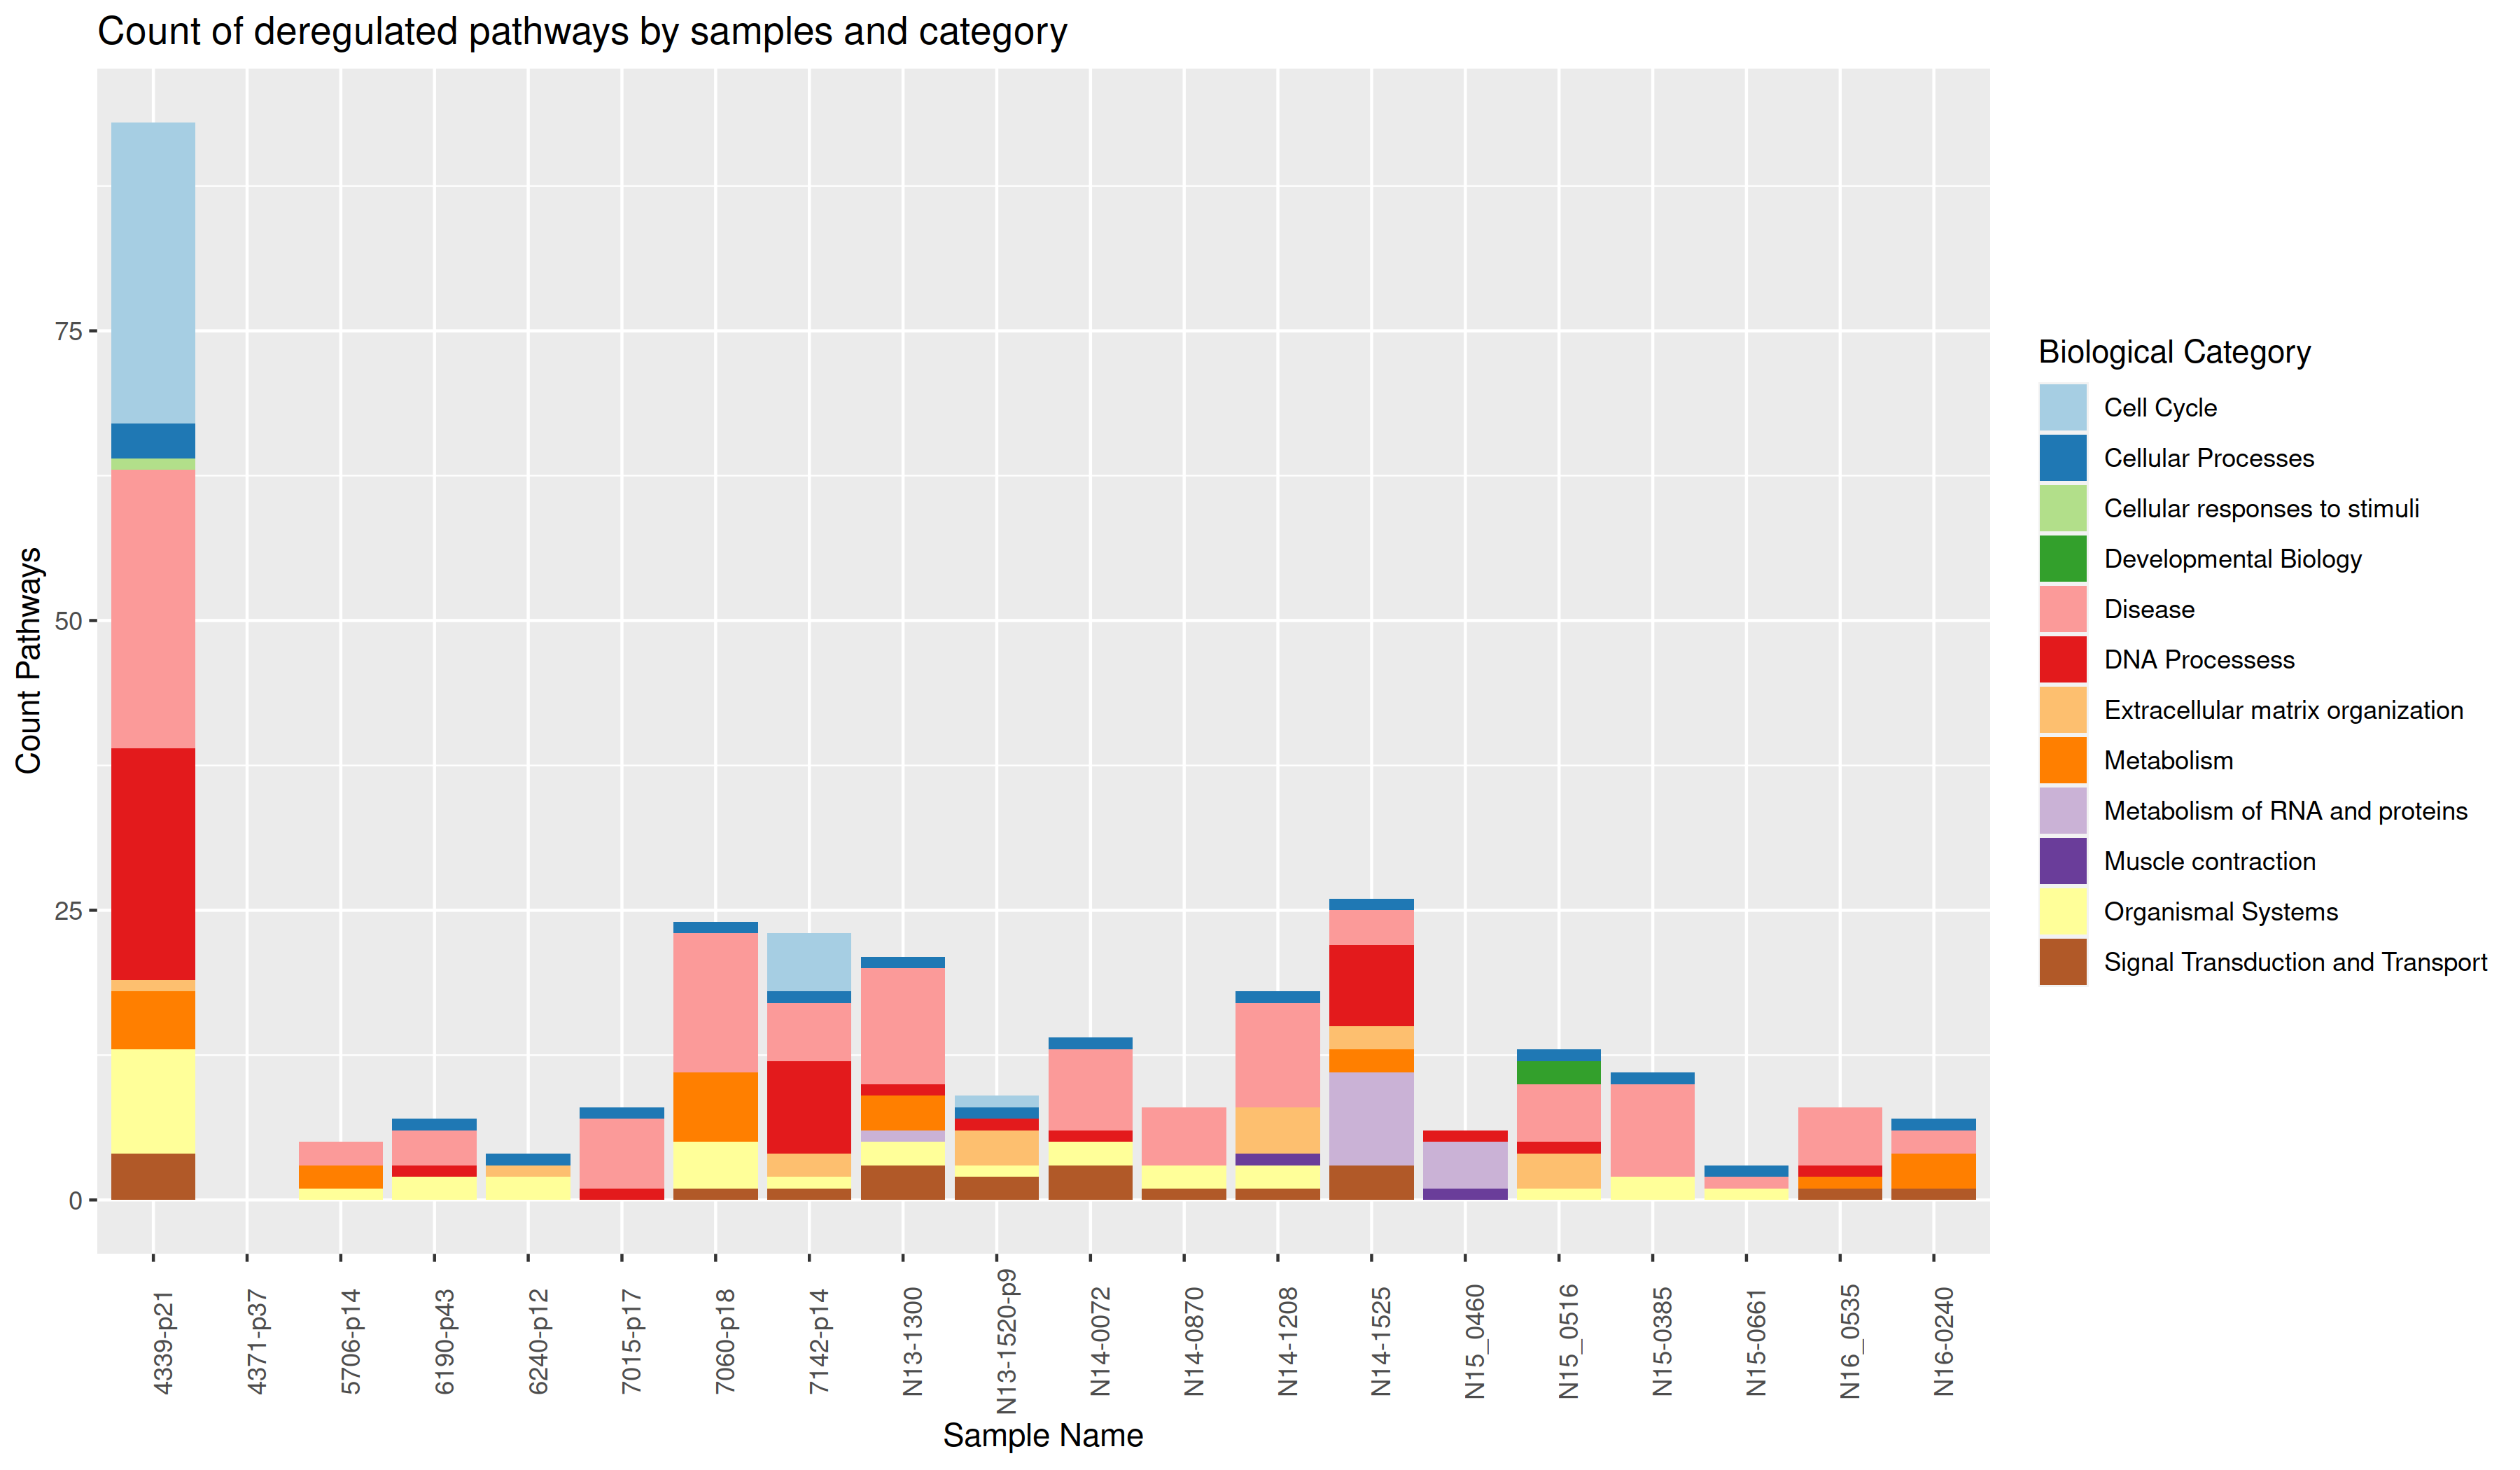
\includegraphics[width=\textwidth]{img/barplot-categ-pdcl}
    \caption{
        Number of deregulated pathways per category and per samples in \acrshort{pdcl} datasets.
    }
    \label{fig:barplot-categ-pdcl}
\end{figure}

Even though that pathways were below the significant threshold in G:Profiler and \acrshort{gsea}, one one samples of the \acrshort{pdcl} dataset (4371-p37) has no pathways common to both enrichment method and thus has no pathways found deregulated.
As can be seen in figure \ref*{fig:barplot-categ-pdcl}, the pathways deregulated in the sample 4339-p21 are mainly involved in the Cell-Cycle or DNA processes (DNA repair and replication).
Not only it is the sample with the most deregulated pathways, but it is the sample with the most biological processes taking places in cell cycling affected as well.

\begin{figure}
    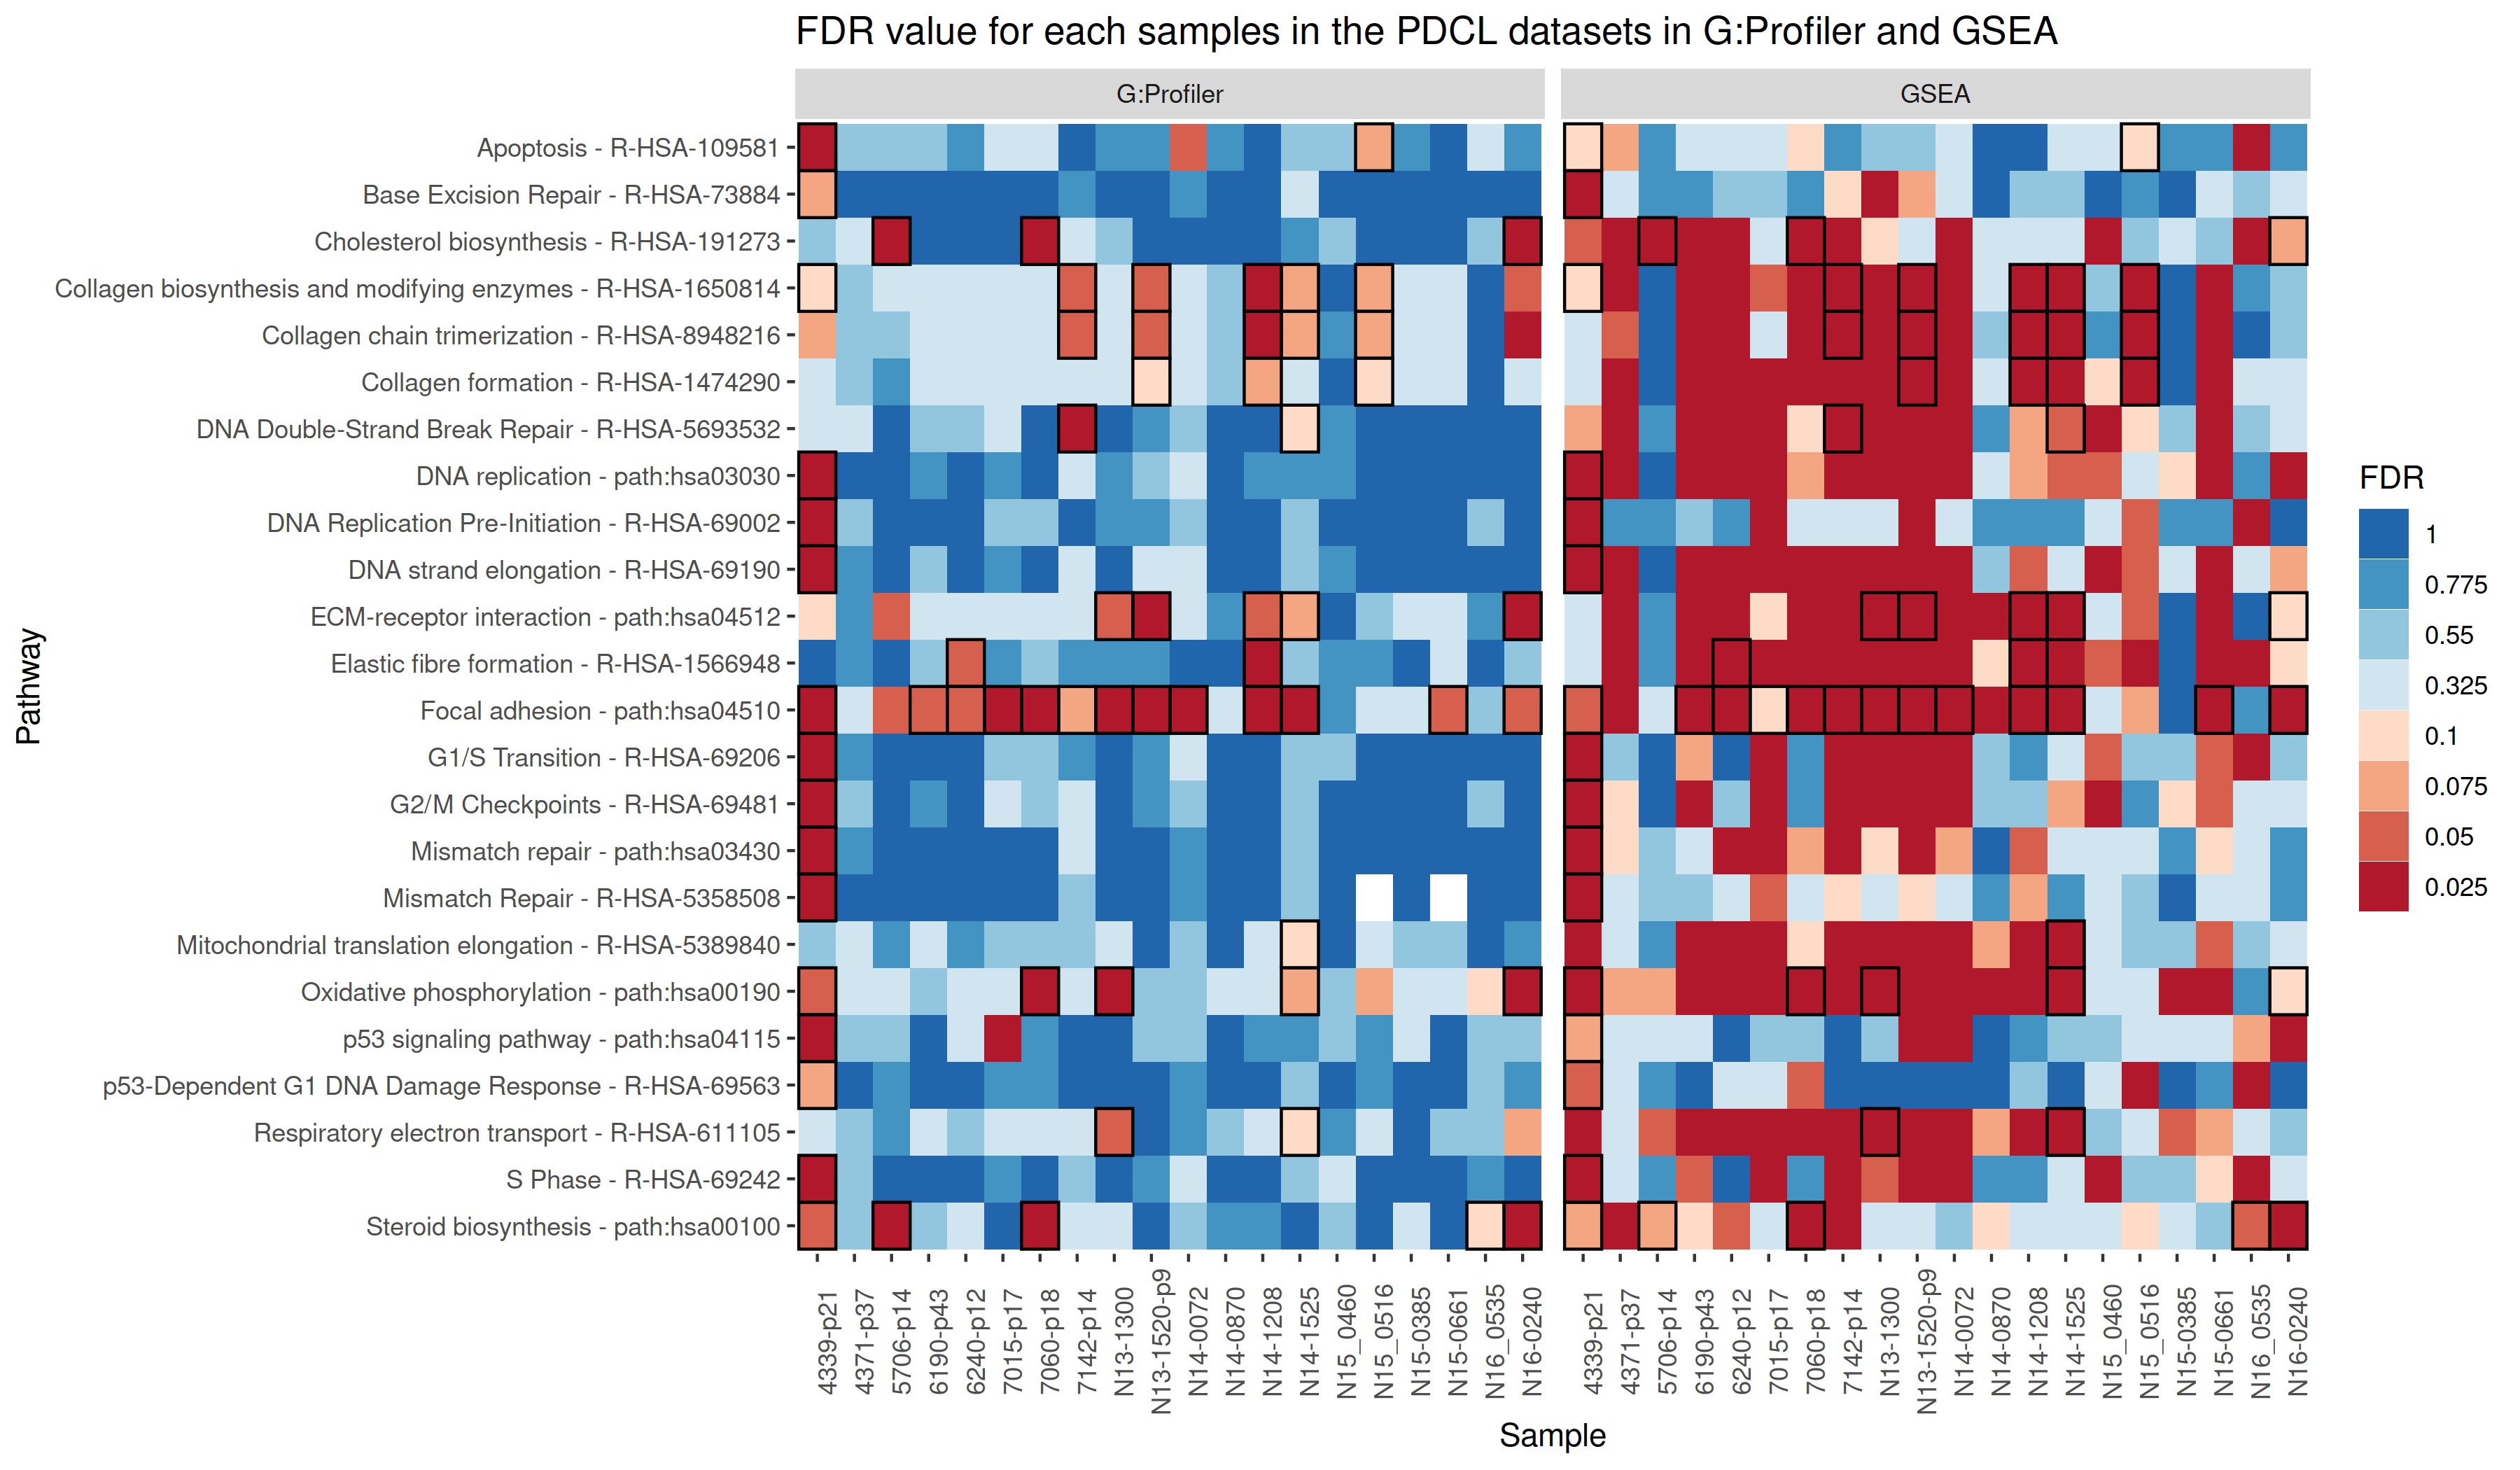
\includegraphics[width=\textwidth]{img/heatmap-fdr-pathway}
    \caption{
        G:Profiler and \acrshort{gsea} \acrfull{fdr} of the pathways deregulated for each samples in the \acrshort{pdcl} datasets.
        Pathways below the significant threshold in both pathway enrichment tools are highlighted in a black box.
        Onhly a selection of pathways are shown in this figure.
    }
    \label{fig:heatmap-fdr-pathway}
\end{figure}

Figure \ref*{fig:heatmap-fdr-pathway} shows that the part of the cell cycle affected for the sample 4339-p21 are the G1/S phases transition, checkpoints in G1 and G2/M phase, DNA repair system and p53 signaling.
p53 is one of the most frequently mutated genes in the case of glioblastoma \cite*{McLendon2008}.
7142-p14 and N14-1525 shows also dysregulation of the \textit{DNA Double-Strand Break Repair} system, despite none of the pathways involved in the different phases of the Cell Cycle are affected.
Samples N13-1300 and N14-1525 are the only samples with a dysregulation in the \textit{Oxidative Phosphorylation} that also present alterations in the \textit{Respiratory electron transport}, N14-1525 showing in addition alteration of the \textit{Mitochondrial translation}, suggesting that they may be different mechanism leading to dysregulated oxidative metabolism.
